% !TEX program = xelatex
% Mixed raster/vector. Source: locked Jan20 2022 author PDF, pp11-14/S3/S5/S6.
% Generated viewports supply illustrations only; equations/arrows are independently checked.
\documentclass[tikz,border=2mm]{standalone}
\usepackage{fontspec,xeCJK,amsmath,amssymb,graphicx}
\setsansfont{Arial}
\setCJKmainfont[Path=/System/Library/Fonts/,BoldFont={STHeiti Medium.ttc}]{STHeiti Light.ttc}
\setCJKsansfont[Path=/System/Library/Fonts/,BoldFont={STHeiti Medium.ttc}]{STHeiti Light.ttc}
\renewcommand{\familydefault}{\sfdefault}
\usetikzlibrary{arrows.meta,calc}
\definecolor{ink}{HTML}{173646}
\definecolor{teal}{HTML}{217E80}
\definecolor{amber}{HTML}{B5712F}
\definecolor{purple}{HTML}{735098}
\definecolor{pale}{HTML}{F6F8F7}
\definecolor{warm}{HTML}{FFF6E9}
\definecolor{violet}{HTML}{F3EFF9}
\tikzset{t/.style={text=ink,font=\fontsize{16.5}{20}\selectfont,align=center,inner sep=0},
 hd/.style={t,font=\bfseries\fontsize{21}{25}\selectfont},
 sm/.style={t,font=\fontsize{15}{18}\selectfont},
 a/.style={-{Stealth[length=3mm,width=2mm]},line width=1.4pt,draw=teal,rounded corners=2pt},
 sup/.style={a,draw=amber,dashed},
 box/.style={rounded corners=4pt,line width=.8pt}}
\newcommand{\txt}[4]{\node[t,text width=#3cm]at(#1,#2){#4};}
\newcommand{\head}[4]{\node[hd,text width=#3cm]at(#1,#2){#4};}
\newcommand{\smalltxt}[4]{\node[sm,text width=#3cm]at(#1,#2){#4};}
\newcommand{\maths}[4]{\node[text=ink,font=\fontsize{#3}{#3}\selectfont,inner sep=0]at(#1,#2){\(\displaystyle #4\)};}
\newcommand{\panel}[7]{\draw[box,draw=#6!45,fill=#7](#1,#2)rectangle++(#3,#4);\pgfmathsetmacro{\pw}{#3-.3}\head{#1+#3/2}{#2+.47}{\pw}{#5}}
% Source PNG has 1536x1024 pixels and 72dpi natural size. Unmodified viewports.
\newcommand{\art}[7]{\begingroup\pgfmathsetmacro{\bt}{1024-#2-#4}\pgfmathsetmacro{\rt}{1536-#1-#3}
\node[anchor=north west,inner sep=0]at(#5,#6){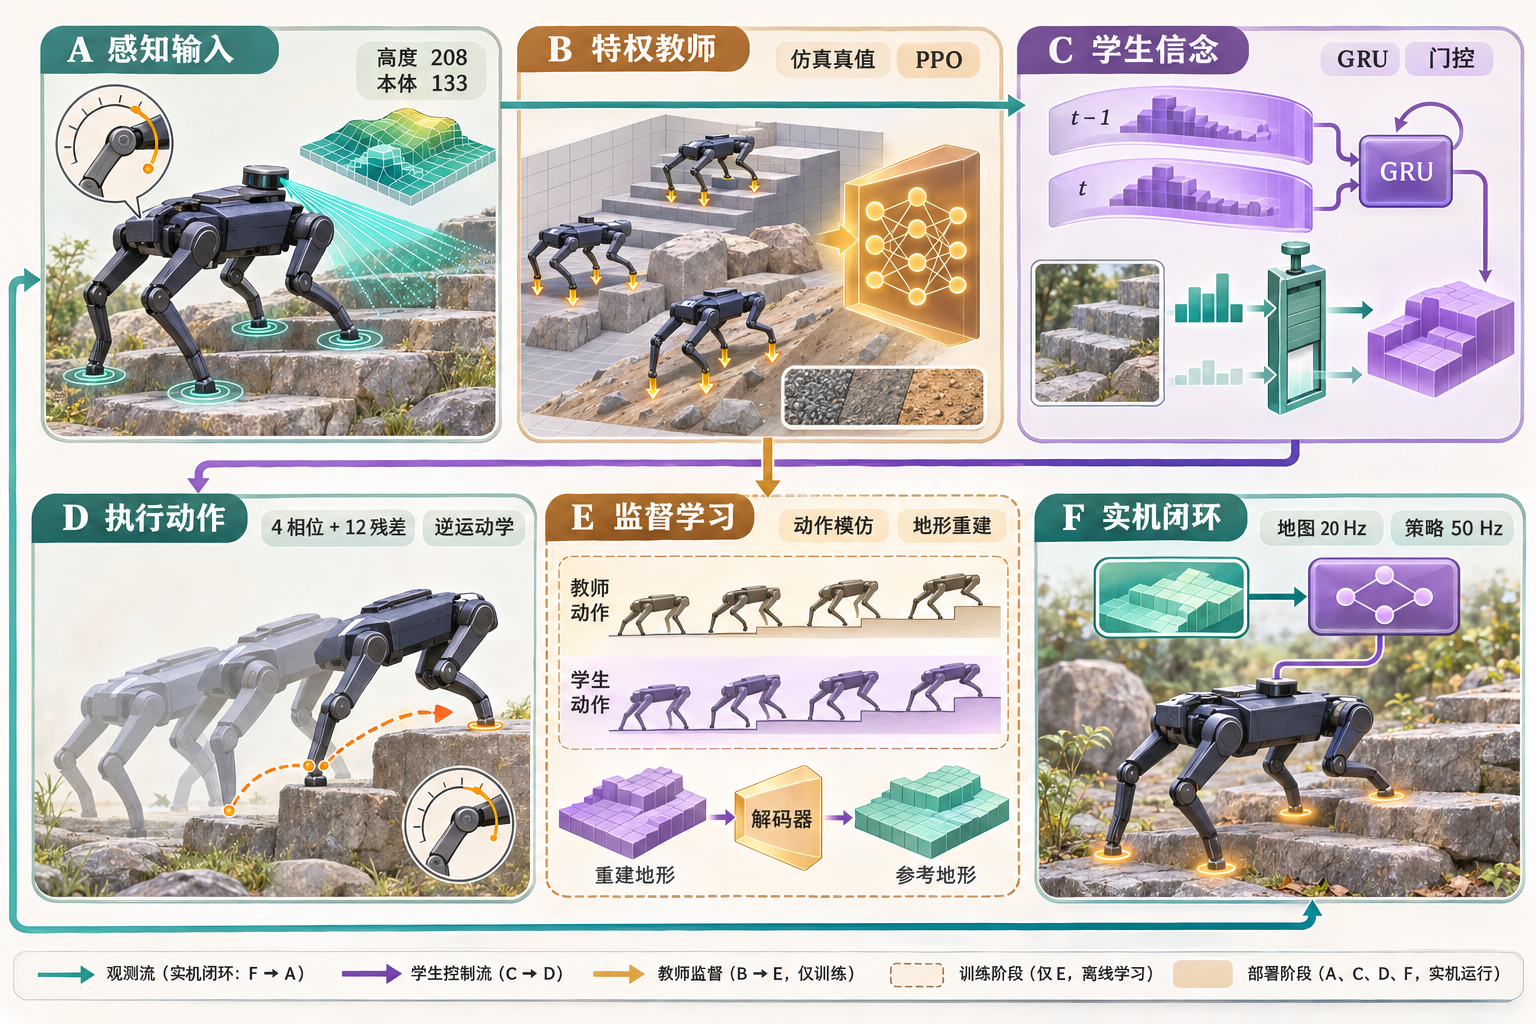
\includegraphics[trim=#1bp \bt bp \rt bp #2bp,clip,width=#7cm]{perceptive-loco-imagegen-draft.png}};\endgroup}
\begin{document}
\begin{tikzpicture}[x=1cm,y=-1cm]
\path[use as bounding box](0,0)rectangle(12.5,20.2);\fill[white](0,0)rectangle(12.5,20.2);
\head{6.25}{.5}{12}{C\quad 门控怎样改写信念？}
\art{1048}{86}{289}{144}{.7}{1.15}{5.2}
\art{1173}{241}{164}{168}{7.0}{1.0}{4.5}
\draw[box,draw=teal!50,fill=pale](.4,5.0)rectangle(12.1,7.25);
\txt{6.25}{5.55}{11.2}{带噪高度 208 → 每脚编码 → 特征 96}
\maths{6.25}{6.45}{19}{l_t^e=g_e(\widetilde o_t^e)\in\mathbb R^{96}}
\draw[a](6.25,7.25)--(6.25,7.8);
\draw[box,draw=purple!50,fill=violet](.4,7.8)rectangle(12.1,10.7);
\txt{6.25}{8.38}{11}{GRU：本体 133 + 高度特征 96 + 历史}
\maths{6.25}{9.15}{19}{(b'_t,h_{t+1})=\mathrm{GRU}(o_t^p,l_t^e,h_t)}
\txt{6.25}{10.05}{11}{2 层 × 50 隐藏单元；历史传给下一步}
\draw[a](6.25,10.7)--(6.25,11.25);
\draw[box,draw=purple!50,fill=violet](.4,11.25)rectangle(12.1,16.3);
\maths{6.25}{11.98}{19}{\alpha_t=\sigma(g_a(b'_t))\in(0,1)^{96}}
\txt{6.25}{12.77}{11}{每个特征分别缩放，再补 24 个零}
\maths{6.25}{13.62}{19}{u_t=\operatorname{pad}_{120}(l_t^e\odot\alpha_t)}
\maths{6.25}{14.5}{20}{b_t=g_b(b'_t)+u_t\in\mathbb R^{120}}
\txt{6.25}{15.45}{11.1}{当前感知与历史估计相加，成为信念}
\draw[a](6.25,16.3)--(6.25,16.85);
\maths{6.25}{17.5}{20}{a_t^S=\pi_S([o_t^p,b_t])\in\mathbb R^{16}}
\draw[box,draw=teal!30,fill=pale](.4,18.3)rectangle(12.1,19.9);
\txt{6.25}{19.1}{11.1}{门只调节直连支路。\quad 带噪高度仍输入 GRU；门值也不是校准概率。}
\end{tikzpicture}
\end{document}
